\begin{enumerate}
\item CSV file from a museum, containing 2433 records of artworks by 197 artists.

\item Linked Data created from the Smithsonian American Art Museum (SAAM) content management system including over 40,000 artworks and 8,000 artists. 
The Linked Data is accessible on a \sparql endpoint.
In previous work~\cite{Szekely:2013vq} ~\todo{cite saam-lod github} we mapped the SAAM dataset to the CIDOC CRM ontology~\cite{Doerr:2003:CCR:958671.958678}, producing a collection of \rtworml mapping files for 14 tables in the SAAM collection management system.
In the demonstration, we are using the SAAM LOD as a proxy for the Linked Data cloud to illustrate the vision of a Linked Data cloud populated with \rtworml models.

\item \rtworml repository containing \rtworml mappings downloaded from the Web and stored in a triple store accessible on a \sparql endpoint (separate from the Linked Data endpoint).
\karma provides a model manager component to manage the \rtworml repository (Fig~\ref{fig:model-manager-screenshot}).
\end{enumerate}
%

\begin{figure*}[bth]
\begin{center}
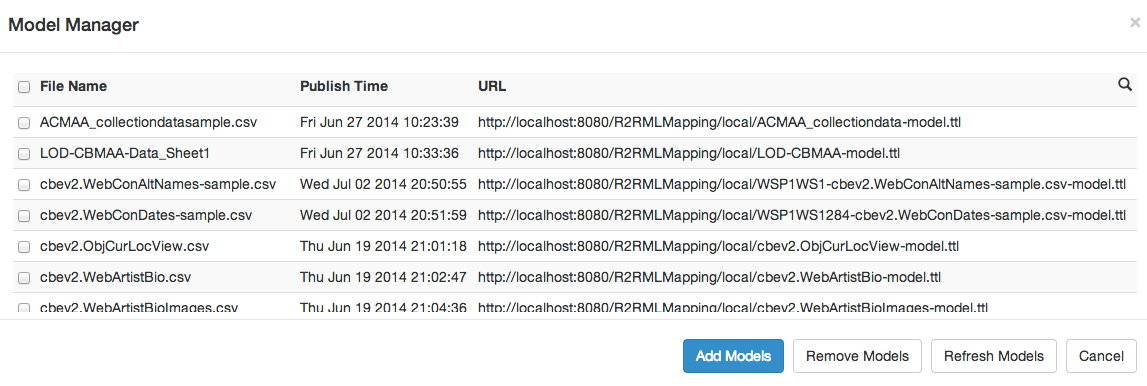
\includegraphics[width=4.8in]{images/3-model-manager.png}
\vspace{-3mm}
\caption{Screenshot of the model manager, showing the \rtworml mappings fetched from the GitHub repository where we shared the mappings for the SAAM dataset}
\vspace{-2mm}
\label{fig:model-manager-screenshot}
\end{center}
\vspace{-1.5em}
\end{figure*}